\section{Analyse Szenarien}
Die Szenarien um die Laufzeitanalyse in dieser Thesis zu dokumentieren, werden in mehrere
bereiche unterteilt sein. Zuallerst werden Tabellarisch, kleinere Code segmente sowohl in Blazor als
auch Qt aufgelistet. Danach werden größere Datenstrukturen mit einer variablen Anzahl an Daten
befühlt. Dabei werden die folgenden drei Datenstrukturen verwendet:

\begin{itemize}
    \item Tabelle
    \item Baum
    \item Chart-Diagram
\end{itemize}

\subsection{Code-Segmente}
\label{subsec:CodeSegemente}
Im folgendem werden 9 Szenarien aufgeführt. Da sich jedoch die Technologien Blazor und Qt stark
unterscheiden, konnte nicht immer die gleiche Struktur angewendet werden. So kam es dazu,
dass hierbei auf das gleiche Verhalten geachtet wurde, als auf die Programmierstruktur. Aus
diesem Grund unterscheiden sich die folgenden Szenarien sehr, führen jedoch zum gleichen Ergebniss.
\newline
\newline
\textbf{Szenario \#1}
\newline
Erzeugen einer neuen leeren ComboBox auf der Benutzeroberfläche.

\begin{zitat}
    \textbf{Blazor Code:}
    \newline
    string widget = @\" <select></select>";
    \newline
    myMarkup = new(widget);
\end{zitat}

\begin{zitat}
    \textbf{Qt Code:}
    \newline
    QComboBox* widget = new QComboBox();
    \newline
    ui->verticalLayout->addWidget(widget);
\end{zitat}
\newline
\newline

\textbf{Szenario \#2}
\newline
Erzeugen eines neuen Labels auf der Benutzeroberfläche.

\begin{zitat}
    \textbf{Blazor Code:}
    \newline
    string widget = @"<label>Text</lable>";
    \newline
    myMarkup = new(widget);
\end{zitat}

\begin{zitat}
    \textbf{Qt Code:}
    \newline
    QLabel* widget = new QLabel("Text");
    \newline
    ui->verticalLayout->addWidget(widget);
\end{zitat}
\newline
\newline

\textbf{Szenario \#3}
\newline
Erzeugen eines neuen Buttons auf der Benutzeroberfläche.

\begin{zitat}
    \textbf{Blazor Code:}
    \newline
    string widget = @"<button>Text</button>";
    \newline
    myMarkup = new(widget);
\end{zitat}

\begin{zitat}
    \textbf{Qt Code:}
    \newline
    QPushButton* widget = new QPushButton("Text");
    \newline
    ui->verticalLayout->addWidget(widget);
\end{zitat}
\newline
\newline

\textbf{Szenario \#4}
\newline
Erzeugen einer neuen Checkbox auf der Benutzeroberfläche.

\begin{zitat}
    \textbf{Blazor Code:}
    \newline
    string widget = @"<input type='checkbox'></input>";
    \newline
    myMarkup = new(widget);
\end{zitat}

\begin{zitat}
    \textbf{Qt Code:}
    \newline
    QCheckBox* widget = new QCheckBox();
    \newline
    ui->verticalLayout->addWidget(widget);
\end{zitat}
\newline
\newline

\textbf{Szenario \#5}
\newline
Erzeugen einer neuen Textbox auf der Benutzeroberfläche.

\begin{zitat}
    \textbf{Blazor Code:}
    \newline
    string widget = @"<input type='text'></input>";
    \newline
    myMarkup = new(widget);
\end{zitat}

\begin{zitat}
    \textbf{Qt Code:}
    \newline
    QTextEdit* widget = new QTextEdit();
    \newline
    ui->verticalLayout->addWidget(widget);
\end{zitat}
\newline
\newline

\textbf{Szenario \#6}
\newline
Erzeugen einer neuen Combobox mit fünf Elementen auf der Benutzeroberfläche.

\begin{zitat}
    \textbf{Blazor Code:}
    \newline
    string widget = @"<select>
    \newline
    <option value='0'>Text1</option>
    \newline
    <option value='1'>Text2</option>
    \newline
    <option value='2'>Text3</option>
    \newline
    <option value='3'>Text4</option>
    \newline
    <option value='4'>Text5</option>
    \newline
    </select>";
    \newline
    myMarkup = new(widget);
\end{zitat}

\begin{zitat}
    \textbf{Qt Code:}
    \newline
    QComboBox* widget = new QComboBox();
    \newline
    widget->insertItem(0, QString::fromStdString("Text1"));
    \newline
    widget->insertItem(1, QString::fromStdString("Text2"));
    \newline
    widget->insertItem(2, QString::fromStdString("Text3"));
    \newline
    widget->insertItem(3, QString::fromStdString("Text4"));
    \newline
    widget->insertItem(4, QString::fromStdString("Text5"));
    \newline
    ui->verticalLayout->addWidget(widget);
\end{zitat}
\newline
\newline

\textbf{Szenario \#7}
\newline
Den Text von einer Textbox lesen.

\begin{zitat}
    \textbf{Blazor Code:}
    \newline
    string textToRead = string.Empty;
    \newline
    <input type="text" @bind-value="@textToRead" />
    \newline
    var text = textToRead;
\end{zitat}

\begin{zitat}
    \textbf{Qt Code:}
    \newline
    auto text = ui->textEdit->toPlainText();
\end{zitat}
\newline
\newline

\textbf{Szenario \#8}
\newline
Den Text eines Labels verändern.

\begin{zitat}
    \textbf{Blazor Code:}
    \newline
    string textToWrite = string.Empty;
    \newline
    <label>@textToWrite</label>
    \newline
    textToWrite = "Text";
\end{zitat}

\begin{zitat}
    \textbf{Qt Code:}
    \newline
    ui->lblTextlabel->setText(QString::fromStdString("Text"));
\end{zitat}
\newline
\newline

\textbf{Szenario \#9}
\newline
Den Text einer Textbox verändern.

\begin{zitat}
    \textbf{Blazor Code:}
    \newline
    string textToWrite = string.Empty;
    \newline
    <input type="text" @bind-value="@textToWrite" />
    \newline
    textToWrite = "Text";
\end{zitat}

\begin{zitat}
    \textbf{Qt Code:}
    \newline
    ui->textEdit->setText(QString::fromStdString("Text"));
\end{zitat}

Von den oben gegebenen Code Segmenten resultieren folgende Ergebnisse. Die Ergebnisse werden in
Mikrosekunden angegeben.

\begin{figure}[h]
    \centering
    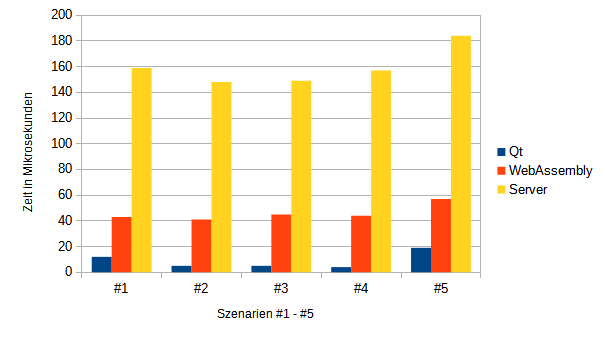
\includegraphics[width=0.9\textwidth, center]{Analyse/Szenarien1_5}
    \caption[Ergebnisse der Szenarien \#1 - \#5 in Microsekunden]{Ergebnisse der Szenarien \#1 -
    \#5
    in Microsekunden}
    \label{img:Szenarien1_5}
\end{figure}
\newline
\newline
\begin{figure}[h]
    \centering
    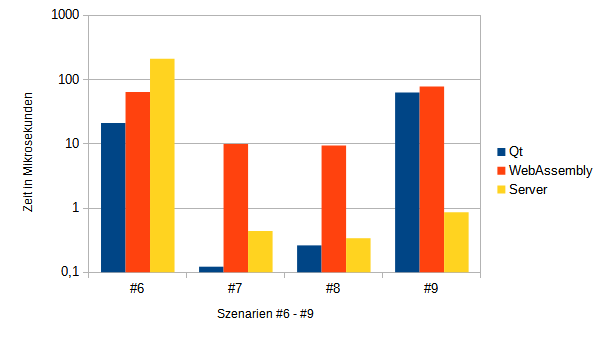
\includegraphics[width=0.9\textwidth, center]{Analyse/Szenarien6_9}
    \caption[Ergebnisse der Szenarien #6 - #9 in Microsekunden]{Ergebnisse der Szenarien #6 - #9
    in Microsekunden}
    \label{img:Szenarien6_9}
\end{figure}
\newpage